
\documentclass[14pt]{extarticle}
\usepackage{amsmath,amssymb}
\usepackage{float}
\usepackage{listings}
\usepackage{multirow}
\lstset{
    %numbers=left,
    breaklines=true,
    tabsize=2,
    basicstyle=\ttfamily,
    literate={\ \ }{{\ }}1
}

\usepackage{graphicx}
\usepackage[T1]{fontenc}
\usepackage{hyperref}
\usepackage[utf8]{inputenc}
\usepackage{geometry}
 \geometry{
 a4paper,
 total={170mm,257mm},
 left=20mm,
 top=20mm,
 }

\usepackage{changepage}
\usepackage{tikz}
\usetikzlibrary{positioning}

%Legend
%\vspace{10pt} interlinea nome section - testo o Titolo elenco - descrizione elenco (Variable) 
\def\sp{\vspace{5pt}}
%\vspace{25pt} interlinea tra sections (Variable)
\def\ss{\vspace{25pt}}
%\vspace{3pt} interlinea tra linee in un paragrafo + breakline (Variable)
\def\pp{\vspace{10pt}\newline}
\def\ppn{\vspace{10pt}}
%Tab 
\def\tab{\hspace*{15pt}}

\usepackage{CJKutf8}
\newcommand{\zh}[1]{\begin{CJK}{UTF8}{gbsn}#1\end{CJK}}

%debug 1 -> debug, 0 -> finale
\newcounter{debug}
\setcounter{debug}{1}

\begin{document}
\title{title}
\author{author}
\date{date}

\begin{titlepage}
	\begin{figure}[t]
    		\centering
\includegraphics[width=0.45\textwidth]{./Image/tongji-university1.png}
    		\centering
\includegraphics[width=0.45\textwidth]{./Image/polito_logo_2021_blu_resized.png}
		\vspace{10mm}
	\end{figure}

	\begin{center}
	    	\textbf{ \LARGE{Tongji University\\}}
		%\textnormal{ \Large{Dipartimento di Automatica e Informatica Collegio di Ingegneria Informatica, del Cinema e Meccatronica\\}}
		\ss
		\textnormal{ \Large {MAURIZIO VASSALLO\\}}
		\textnormal{ \large {Student ID: \\}}
		\textnormal{ \large {Academic Tutor: a\\}}
		%\vspace{30mm}
	    		\vspace{\fill}\textbf{\LARGE{A Collision Avoidance System Using
Reinforcement Learning\\}}\vspace*{\fill}%vertical align
	\end{center}
	
\end{titlepage}

\tableofcontents
\newpage

\begin{center}
	\section{Introduction}
	\sp
\end{center}
\begin{flushleft}
	This report is drawn up after the development of the thesis project at Tongji University (\textbf{\zh{同济大学}}) for the Double Degree project Politong.
	\pp
	The thesis project aims to develop a machine learning algorithm that allows an autonomous vehicle to avoid obstacles. \\
	The research will focus on Reinforcement Learning methods.

\subsection{Autonomous Vehicles Overview}
Nowadays it is possible to hear more and more about Autonomous Driving Vehicles.
The autonomous cars (also known as a self-driving cars or a driverless cars) are a vehicle that are capable of sensing their environment and to navigate without human input.
The ability of autonomous vehicles to operate without human intervention depends
on their level of technological sophistication, in accordance with the current six-degree
autonomy scale proposed by the International Society of Automotive Engineers (\textbf{SAE})\cite{AVtaxonomy}.
There are 6 levels of driving automation, from level 0 (no automation) to level 5 (full unlimited automation); intermidiate levels (1 to 3) are considered semi-autonomous\cite{AVlevels,AVlevels2}. \\
Currently we are between level 2 and 3, so even if the current technology is behind the famous Level 5 of driving automation, there is lot of work to make it happen.

\ppn
According to research firm, autonomous vehicles will match or exceed human safety by late 2020s and fulfill all mobility needs in 2040s to 2060s. Optimists predict that by 2030, autonomous vehicles will be sufficiently reliable, affordable and 
common to displace most human driving, providing huge savings and benefits. However, there are good reasons to be skeptical. There is considerable uncertainty concerning autonomous vehicles development, benefits, costs, travel impacts and consumers demand. Considerable progress is needed before autonomous vehicles can operate reliably in mixed urban traffic, heavy rain and snow, unpaved and unmapped roads, and where wireless access is unreliable\cite{AVfirm}.


\ppn
The idea behind these cars is quite simple: outfit the vehicles with sensors that can track all the objects nearby and make the cars understand the world around them. Autonomous vehicles are driven using technology such as GPS, odometry (usege of data from motion sensors to estimate change in position over time), radars, laser lights and other devices\cite{AVlevels2}. These sensors themselves do not make the car ‘smart’, what make it autonomous are the big computers inside and the algorithms they are running. Usually these softwares run neural networks: these take as input the sensor recordings, elaborate them and output some values like steering angle, accelerate, brake or other important values. Even if the idea behind these technological innovative vehicles is simple the implementation is not so straightforward, for some reasons: not enough hardware computation, not enough training data, problems with handle different weather conditions (fog, rain, snow, etc.),  the current regolation remains in a nascent stage.
 \pp
Even if this tecnology is not diffused yet, there are many potential benefits that autonomous vehicles could introduce in our society:
 \begin{itemize}
 \item \textbf{Transportation Safety}. The most notable predicted benefit of autonomous vehicle technology is a substantial reduction in the human and economic toll of traffic accidents. Indeed, impairment, distractions, and fatigue alone account for over 50\% of all fatal crashes. The use of autonomous vehicles could significantly reduce the incidence of such crashes, as vehicles with no-human operators are never drunk, distracted, fatigued, or otherwise susceptible to human failings.
\item \textbf{Access to Transportation}. Another important potential benefit of autonomous vehicle technology is increased mobility for populations currently unable or not permitted to operate traditional vehicles. These populations include older
citizens, disabled, people too young to drive and people without a driver’s 
license.
\item \textbf{Traffic Congestion and Land Use}. Autonomous vehicles could reduce congestion and change the way in which cities are planned. Most car are moving only for 5\% of their lives, for the 95\% they are parked\cite{AVparking}! For this reason lot of space is dedicated to parking lots; the same space that could be used for different purposes (green spaces, etc.).
\item \textbf{Energy and Emissions}. Autonomous vehicle technology has the potential to reduce both energy consumption and pollution thanks to efficiencies gained through smoother acceleration and deceleration and  increased  roadway capacity.\cite{AVbenefit}
 \end{itemize}
 
 To do: find a way to link this part with teh following one!!

	\ss
\end{flushleft}

\newpage
\begin{center}
	\section{Reinforcement Learning}
\end{center}

\subsection{Introduction}
\sp
\begin{flushleft}
Humans and animals learn through a process of trial and error. This process is based on a reward mechanism that provide a response to our behaviors. The goal of this process is to incentivize the repetitions of actions which trigger positive rewards and disincentivize the repetition of actions which trigger negative ones.
\\
Inspired by how animals and humans learn, \textbf{Reinforcement Learning} is built around the idea trial and error from an interaction with the enviroment 
%cite{andrea lonza book}.
\pp
Reinforcement Learning tries to solve the problem in which a decision-maker, Agent, can perform some action inside a world, called Enviroment. The agent senses the enviroment through the state and for each state the agent has to perform an action. These actions result in an effect: they change the agent's state and give it a feedback, the Reward. The reward is a value which indicated if the action performed is good, then the reward is positive, or it is bad, the reward is negative. Given these rewards the agent understand what action to perform in a given state to get a positive reward. 
\\
This cycle of state-action-reward is repeted many times. The goal of the agent is to find a policy such that the actions perform lead to the maximum reward possible. In particual the agent wants to maximize the cumulative reward, the sum of rewards over a period of time. The difference between maximizing the instant reward and cumulative reward is an important distinction because: choosing an action which lead to the maximum next reward could in the next state bring to an end state (game over); instead maximizing the cumulative reward means thinking in a long-term horizon, so that the next states should all have a positive reward (even if the action chosen in one state is not the one that the
maximum next reward).

\subsection{Reinforcement Learning compared to other methods}
Machine learning is the science of getting computers to act without being explicitly programmed. Machine Learning methods are appropriate in application settings where
people are unable to provide precise specifications for desired program behavior, but
where examples of desired behavior are available, or where it is possible to assign a
measure of goodness to examples of behavior\cite{RLandSL}.
\\
There are mainly 3 methods to train Machine Learning algorithms, each with its advantages and disavantages. The 3 methods are:
\begin{itemize}
\item Supervised Learning. In this method the algorithm is trained with labeled data; the training examples are of the form ($x_i$,$y_i$), with $x_i$ a \emph{n-dimentional} vector and $y_i$ a scalar (it can represent either a class or a floating value). The learner (either a classifier or a predictor) tries to find a good mapping fuction that maps an input $x_i$ to its correspoding $y_i$. During this learning process the error between the $y_i$ predicted and the actuall value is calculated and used to make the method learning (usually with Gradient Descent and Back Propagation) and decresing the error over time. A popular example is to classify and image given the raw pixels.
\item Unsupervised Learning. The main difference between Unsupervised Learning and Supervised Learning is that in the former method data does not have labels. In this setting, the goal is usually find the relationship in the elements of the dataset. This is done calculating the distance (Euclidian, Hamming, etc.) between the points: if the distance between the points is small, they may share similar characteristics. A popular example is detecting a person purchase preferences analyzing his shopping list with other people shopping's lists.
\item Reinforcement Learning. Reinforcement Learning comes into play when examples of desired behavior are not available but where it is possible to score examples of behavior according to some performance criterion\cite{RLandSL}. In general, in Reinforcement Learning the goal is to maximized an unknown reward fuction through and trial and error process. A popular example is a car that learns to drive in a given enviroment with no prior knowledge given.
\end{itemize}
Supervised and Reinforcement Learning could be considered similar but there are few key differences, in particual the goal in Supervised Learning is to predict the right label while in Reinforcement Learning the goal is to find an action $x^*$ in other to maximized the reward. For this reason instead of minimizing the error between the predicted class and the real class, the goal is to choose an action that maximize the cumulative reward in a given state.

\subsection{Application of Reinforcement Learning}
Some possible application of RL:
\begin{itemize}
\item Self-driving cars. Train a car in a real world can be dangerous (people can be hurt) and expensive (car can hit an object and damage the vehicle). They can be trained in a RL setting: the car is the agent, the world around it the enviroment, it has to take some actions (throttle, steer, etc.), the state are the sensors and the goal is to reach a destination avoiding obstacles. In this setting the agent can get positive or negative rewards depending on the action chosen.
\item Games. Popular example are: chess, Go and Dota. In all these games computers were able to beat the champions.
\item Finance. Many problems can be formulated as a RL problem, for example the stock trading. Here the action could be: selling, buying, holding and the goal is to maximize the  cumulative return over a period of time.
\item many other applications\cite{RLapplications}.
\end{itemize}

\subsection{Formal definition}
\sp
Reinforcement Learning can be formulated as a Markov Decision Process (MDP), indeed a MDP express the problem of sequential decision-making, where for each state $s$ the dicision maker can choose any action $a$ available in that state $s$. The process respond moving with some probability to the state $s^\prime$ and giving the decision maker a reward $R_a(s,s^\prime)$ (read as: `the reward given when in state $s$ and the action $a$ chosen brings to the next state $s^\prime$')
\\
The MDP is defined as a tuple of 4 elements (S, A, P, R), where:
\begin{itemize}
\item S is a set of states, called the \emph{state space}.
\item A is a set of actions, called the \emph{action space}.
\item P is the probability from state $s$, at time $t$, of reaching state $s^\prime$, at time $t+1$ with action $a$:
\[P_a(s,s^\prime) = Pr(s_{t+1} = s^\prime | s_t = s, a_t = t)\]
\item $R_a(s,s^\prime)$ is the immediate reward received after transitioning from state $s$ s to state $s^\prime$, due to action $a$.
\end{itemize}
The state and action spaces may be finite or infinite.

\ppn
The MDP is controlled by a sequence of descrete time steps that create a trajectory $\upsilon$:
\[s_0 \xrightarrow{a_0} s_1 \xrightarrow{a_1} s_2 \xrightarrow{a_2} s_3 \xrightarrow{a_3} \dotso\]
where the states follow the state transition $P_a(s,s^\prime)$. The transition function and the reward function are determined only by the current state, and not from the previous states. This property is called Markov property, which is a characterize the MDP and it means that the process is memory-less and that the future states depends only on the current one and not on its history.

\ppn
The goal of the MDP is to find a good policy for the decision maker: a function $\pi$ that specifies the action $\pi(s)$ that will be chosen when in state $s$. The policy $\pi$ found will maximize the cumulative reward over a trajectory $\upsilon$:
\[ G(\upsilon) = \sum_{t=0}^{\infty} R_{a_t}(s_t, s_{t+1}) \] 
%R_{a_0}(s_0, s_{1}) + R_{a_1}(s_1, s_{2}) + \dotso =
This return value has the problem that all the rewards contribute in the same weight and this can create some problems due to the lack of information. A better return value would be to give some more importance to the short-term memories and giving less importance to the one far in the future. This is solved introducing a \textbf{discount factor}, denoted with $\gamma$. Then the corrected formula is:
\[ G(\upsilon) = \sum_{t=0}^{\infty} \gamma^t R_{a_t}(s_t, s_{t+1}) \]
with value of $\gamma$ satisfying $ 0 \leq \gamma \leq 1$. A lower discount factor motivates the decision maker to take actions that are close in time instead of actions that a far in the future.

\ppn
%http://incompleteideas.net/book/ebook/node34.html
%https://cims.nyu.edu/~donev/Teaching/WrittenOral/Projects/XintianHan-WrittenAndOral.pdf
Another important notion in MDP and Reinforcement Learning is the value fuction. While the return $G(\upsilon)$ gives the reward over a trajectory it does not tell much about how good are the single states. The value fuction does exactly this, it estimates how good is for the decision maker to be in a given state. The notion of "how good" is defined in terms of future rewards that can the decision maker expect in terms of expected return.
\\
The value fuction $V_{\pi}(s)$ can be formally defined as: 
\[V_{\pi}(s) = \mathbb{E}_{\pi}(R_t|s_t=s) = \mathbb{E}(\sum_{t=0}^{\infty} \gamma^t R_{a_t}(s_t, s_{t+1})|s_t=s)\]
\vspace{-9.3mm}
\begin{center}
The expected return when starting at state $s$ and following policy $\pi$.
\end{center}

Similary, another notion: the action-value fuction, the expected return from state $s$ with an initial action $a$:
\[Q_{\pi}(s,a) = \mathbb{E}_{\pi}(R_t|s_t=s, a_t=a) = \mathbb{E}(\sum_{t=0}^{\infty} \gamma^t R_{a_t}(s_t, s_{t+1})|s_t=s,a_t=a)\]

Furthermore, the value fuction and the action-value fuction are called V-fuction and Q-fuction. They are related and satisfy a particular relationship, used in many Reinforcement Learning contests, that for any policy $\pi$ and state $s$, the following condition holds:
\[V_{\pi}(s) = \mathbb{E}_{\pi}(Q_{\pi}(s,a))\]

\ppn
The V-fuction can be decomposed in 2 terms:
\begin{equation} \label{eq:1}
V_{\pi}(s) = \mathbb{E}_{\pi}(R_t|s_t=s) = 
					\underbrace{\mathbb{E}_{\pi}(R_{t}|s_t=s)}_{\text{immidiate reward}} + 
					\underbrace{\mathbb{E}_{\pi}(\gamma V_{\pi}(s_{t+1}|s_t=s))}_{\text{discounted value of next state}}
\end{equation}
This is the Bellman Equation (\ref{eq:1}) that defines the value fuction recursively, enabling the estimations of the next states. \\
Similary it is possible to write Bellman equation for the Q-fuction :
%(using the V-fuction and Q-fuction relationship)
\[Q_{\pi}(s,a) = \mathbb{E}_{\pi}(R_t|s_t=s, a_t=a) = \mathbb{E}_{\pi}[R_t + \gamma Q_{\pi}(s_{t+1},a_{t+1})| s_t=s, a_t=a] \]
In this way the V-fuction and the  Q-fuction are updated with the values of the successive states without the need to know the trajectory till the end.

\subsection{Q-Learning}
\sp
Q-learning is an off-policy reinforcement learning algorithm that tries to find the best action to take given the current state. It's considered off-policy because the Q-learning function learns from actions that are outside the current policy, like taking random actions and that the updates can be made independently from the policy that has gathered the expirence. In other words, this means that off-policy algorithms can use experiecens collected in the past to improve the policy.\\
Q-Learning is also a TD algorithm (Temporal Difference algorithm\cite{TDl}) and it inherits from the TD learning the characteristics of one-step learning.\\
These two elements (TD and off-policy property) are important; indeed the goal of Q-learning is to approximate the Q-fuction using the action the maximize the Q-value of the next state. Formally:
\begin{equation} \label{eq:2}
 Q(s_t,a_t) = Q(s_t,a_t) + 
\alpha[r_t + \gamma \text{max}_{a}Q(s_{t+1},a) - Q(s_t,a_t)] 
\end{equation}
where $\alpha$ is the learning rate, that indicated how much the Q-value will be updated, and $\gamma$ the discount factor, that, as mentioned, gives more importance to the short-term actions and gives less importance to the long-term ones. \\
This modified version of the Bellman equation updates the value of the current Q-value using only the next step (using the TD one-step learning property) and it is an off-policy 
algorithm since it uses the $\text{max}_{a}$ to choose $a_{t+1}$.

\ppn
Simple Q-learning (also known as Vanilla Q-learning) problems can be solved using a Q-table, where for each state there are all the Q-values for all possible the actions:

\begin{table}[H]
\centering
\begin{tabular}{|c|c|c|c|c|}
\hline
\multirow{2}{*}{\textbf{States}} & \multicolumn{4}{c|}{\textbf{Actions}}                                \\ \cline{2-5} 
                                 & \textbf{$a_1$} & \textbf{$a_2$} & \textbf{$\dotso$} & \textbf{$a_m$} \\ \hline
$s_1$  				& $Q(s_1,a_1)$   				& $Q(s_1,a_2)$  				&  $\dotso$  				& $Q(s_1,a_m)$                \\ \hline
$s_2$  				& $Q(s_2,a_1)$   				& $Q(s_2,a_2)$  				&  $\dotso$  				& $Q(s_2,a_m)$                \\ \hline
$\dotso$      &  $\dotso$              	& $\dotso$              	&  $\dotso$              & $\dotso$              \\ \hline
$s_n$  				& $Q(s_n,a_1)$   				& $Q(s_n,a_2)$  				&  $\dotso$  				& $Q(s_n,a_m)$                \\ \hline
\end{tabular}
\caption{state-action Q-values}
\label{tab:my-table}
\end{table}
with $s_i$ a \emph{t-dimentional} array (imagine a possible car's state which at each instant record $t$ values from different sensors).
During training the Q-values are updated using equation the Bellman equation for Q-learning (\ref{eq:2}).
\\
This implementation has 2 main problems:
\begin{itemize}
\item It is possible to to see that the size of the table increases exponentially with the increasing number of states ($n$) and the number of actions ($m$), increasing the memory required to store the table.
\item The amount of time required to explore each state to create the required Q-table would be increase too.
\end{itemize}
%The space complexity would be $\Omega(t \times n \times m)$!

\ppn
One way to solve this problem is to use a method that approximate the Q-fuction: one possible candidate is to use neural networks, since they are considered universal approximator fuctions. This new architecture assumes the name of \textbf{Deep Q-learning}. Deep Q-learning replaces the Q-table with a neural network that approximate the Q-value fuction; moreover rather than mapping a state-action pair to a Q-value, a neural netowk maps an input state to an \emph{(action, Q-value)}.
\\
This solution overcomes the 2 problems mentioned above.
\pp
In this contest, the objective is to change the neural network's weights $\theta$, so that $Q_{\theta}$ is an optimal Q-value fuction. \\
In order to change the weights, as common with neural networks, the \textbf{Gradient Descend} is employed. In particular the weights are changed with the following formula:
\[ \theta = \theta - \alpha\nabla_{\theta}\mathbb{E}_{(s,a,r,s^\prime)}[(Q_{\theta}(s,a) - \text{target})^2]\]
where:

\begin{equation} \label{eq:target}
\text{target} = r + \gamma\text{max}_{a^\prime}Q_{\theta}(s^{\prime},a^{\prime})
\end{equation}
\vspace{-10mm}
\begin{center}
is the value the neural network should predict;
\end{center}

\[Q_{\theta}(s,a)\]
\vspace{-10mm}
\begin{center}
is the value the neural network prediction;
\end{center}

\[\mathbb{E}_{(s,a,r,s^\prime)}[(Q_{\theta}(s,a) - \text{target})^2\] 
\vspace{-10mm}
\begin{center}
is the average Mean Square Error over a batch iteration;
\end{center}

\[\nabla_{\theta}\]
\vspace{-10mm}
\begin{center}
is the gradient of the loss w.r.t the neural network's weights.
\end{center}

In this way over many interaction the weights are updated to reduce the loss and increase the cumulative reward. 
\end{flushleft}


\newpage
\begin{center}
	\section{Project Development}
	\sp
\end{center}
\begin{flushleft}
	The goal of the project is to use some Reinforcement Learning algorithms to teach an actor to avoid obstacles. The \textbf{Agent} is put in an \textbf{Environment} it does not know and it will learn a good \textbf{Policy} in order to avoid the walls using a trial and error approch. The agent will be given with positive or negative \textbf{Rewards} depending on the \textbf{Actions} it performs. 
	
	\subsection{Environment}
	\sp
	In this project a deterministic environment will be used since the next state of the environment can always be determined based on the current state and the agent’s action. In particular the are 2 main environments:A simple track, and a complex one used for testing purposes. Both track where modelled in \textbf{Blender} version 2.93\cite{Blender}. \\
	These models are used inside of Unreal Engine 4 \cite{UE4}, a powerful game and physics engine.
	
	\subsubsection{Simple Track}
	This simple track is used for training and validation. Since this is used for training it does not have long straightaways or sharp turns.
	\ifnum\value{debug}=0 {
	\begin{figure}[H]
    		\centering
\includegraphics[width=0.45\textwidth]{./Image/Environment/Easy/perspective.png}
    		\centering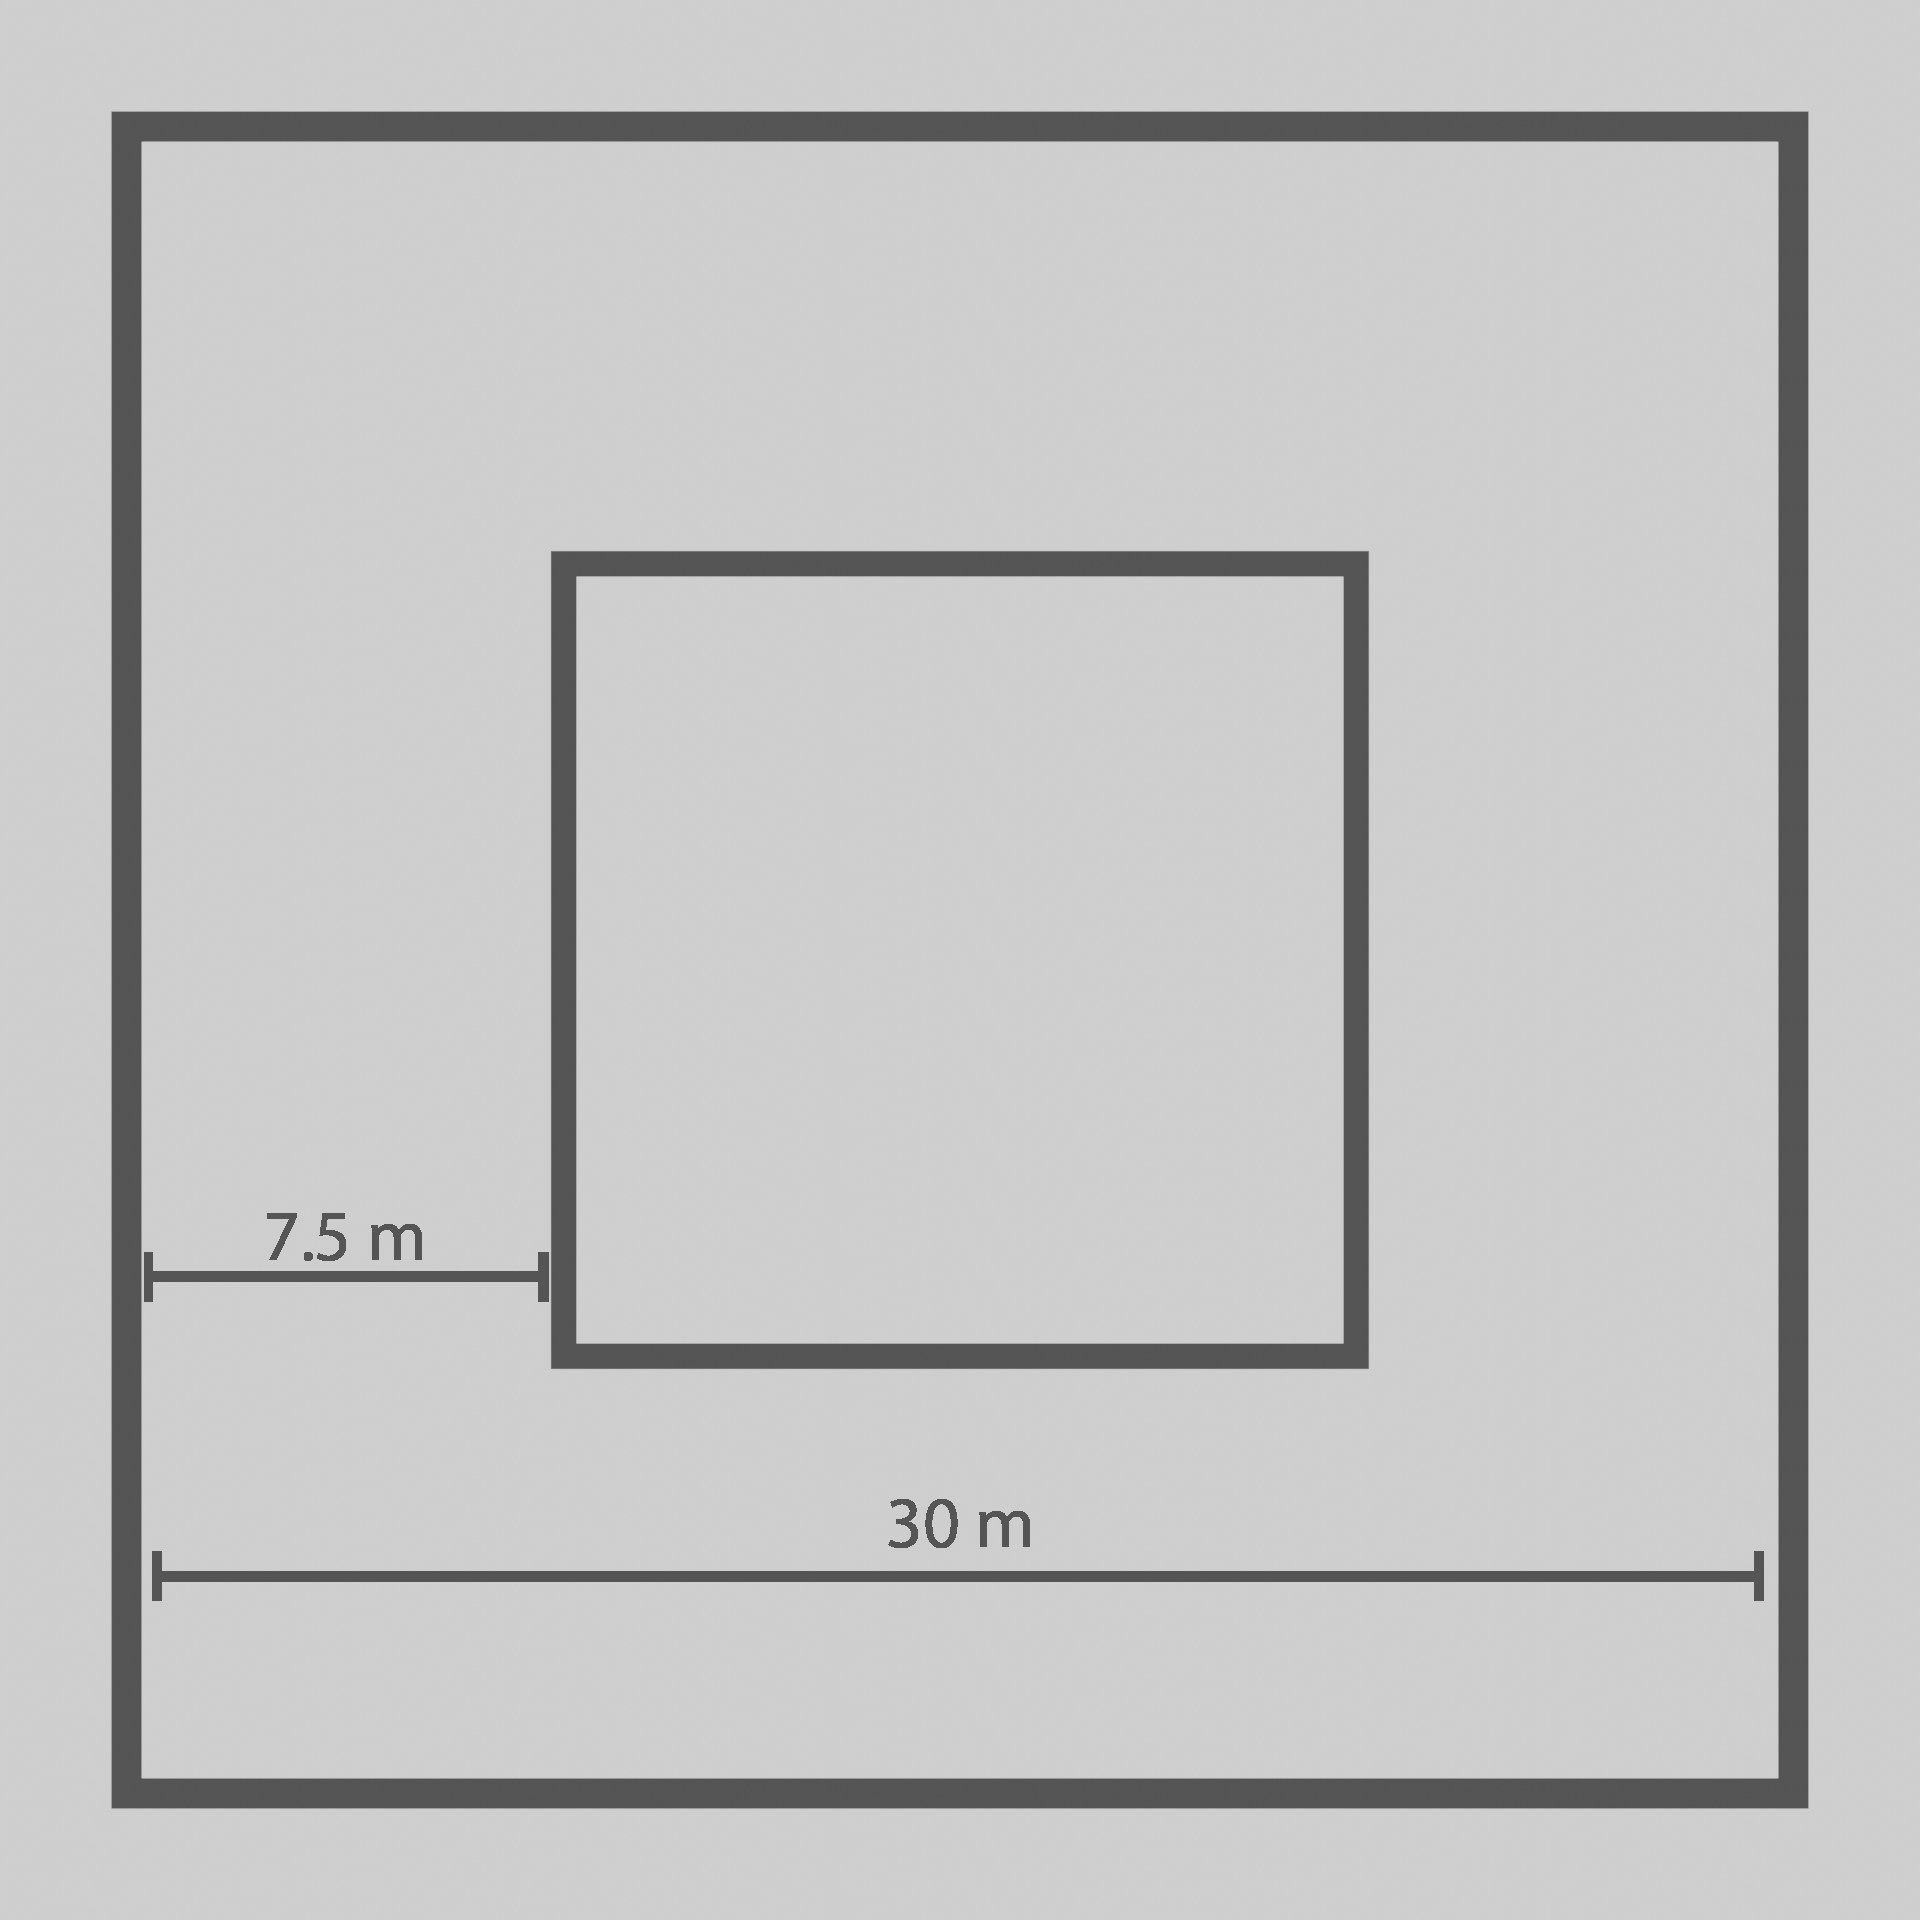
\includegraphics[width=0.45\textwidth]{./Image/Environment/Easy/top_mod.png}
		\vspace{5mm}
		\caption{Simple track images. On the left there is the perspective view and on the rigth the orthogonal top view with its measurings.}
	\end{figure}
	}\fi
	During training the track is run clockwise and counterclockwise so that the agent learns to turn right and left.
	
	\subsubsection{Complex Track}
	This complex track is used for testing. This will have more long straightaways or sharp turns.
	\ifnum\value{debug}=0 {
	\begin{figure}[H]
    		\centering
\includegraphics[width=0.45\textwidth]{./Image/Environment/Med/perspective.png}
    		\centering
\includegraphics[width=0.45\textwidth]{./Image/Environment/Med/top.png}
		\vspace{5mm}
		\caption{Complex track images. On the left there is the perspective view and on the rigth the orthogonal top view with its measurings.}
	\end{figure}
	}\fi
	
	\subsection{Agent}
	\sp
	The agent is a car available on the Vehicle Variety pack \cite{VVp} asset of Unreal Engine 4. From this packet only the `SportCar' content is used and some settings are modified (drag coefficient and other physical values).
	\begin{figure}[H]
    		\centering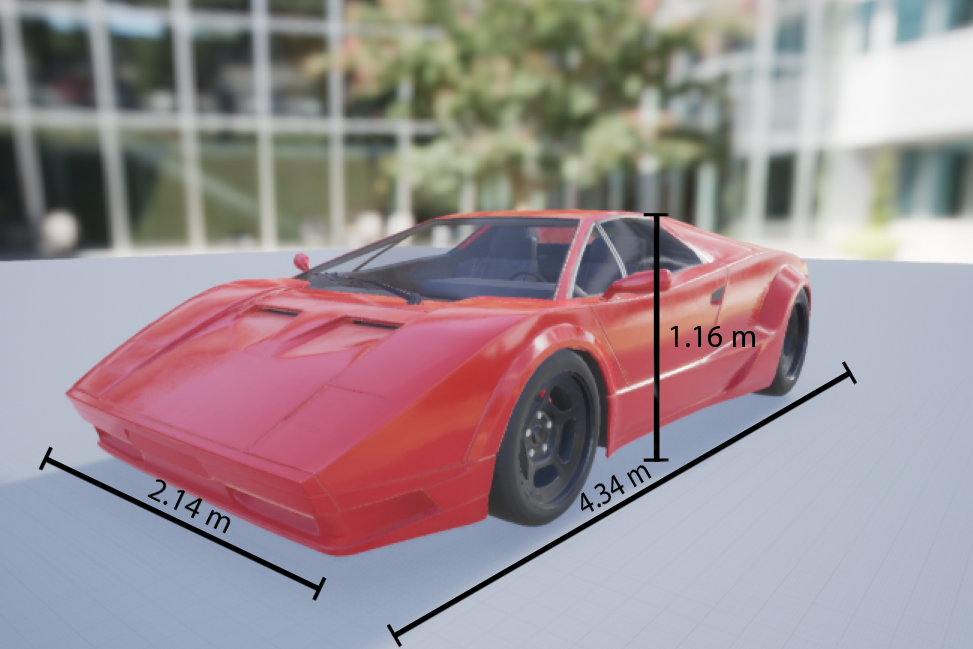
\includegraphics[width=0.7\textwidth]{./Image/Agent/car.png}
		\vspace{5mm}
    		\caption{The used car as Agent with its own measurements}
	\end{figure}
	
	\subsection{State}
	\sp
	The agent senses the environment around it using some LIDAR sensors (light detection and ranging \cite{Lidar}). \\
	The number of Lidar to use is an important hyper-parameter: in this case good results were found using 32 Lidar sensors. This 32 sensors are equally spaces in an angle range of $170^{\circ}$, this is another important hyper-parameter. \\
	Multiple tests were made to set these hypre-parameters, in particular:
	\begin{itemize}
	\item Too many LIDAR sensors requires more training time, they increase the performance but sometimes the model did not converge.
	\item With too few LIDAR sensors the algorithm did not have enough information to learn properly.
	\item Too wide angle decresed the sensor density and decresed the focus on the most important part: the front and the sides of the car.
	\item Too small angle increased the sensor desity and increased the focus only on some specific region: the front.
	\end{itemize}
	So a trade-off between training time and performances were reached with 32 sensors and a $170^{\circ}$ angle
	\ifnum\value{debug}=0 {
	\begin{figure}[H]
    		\centering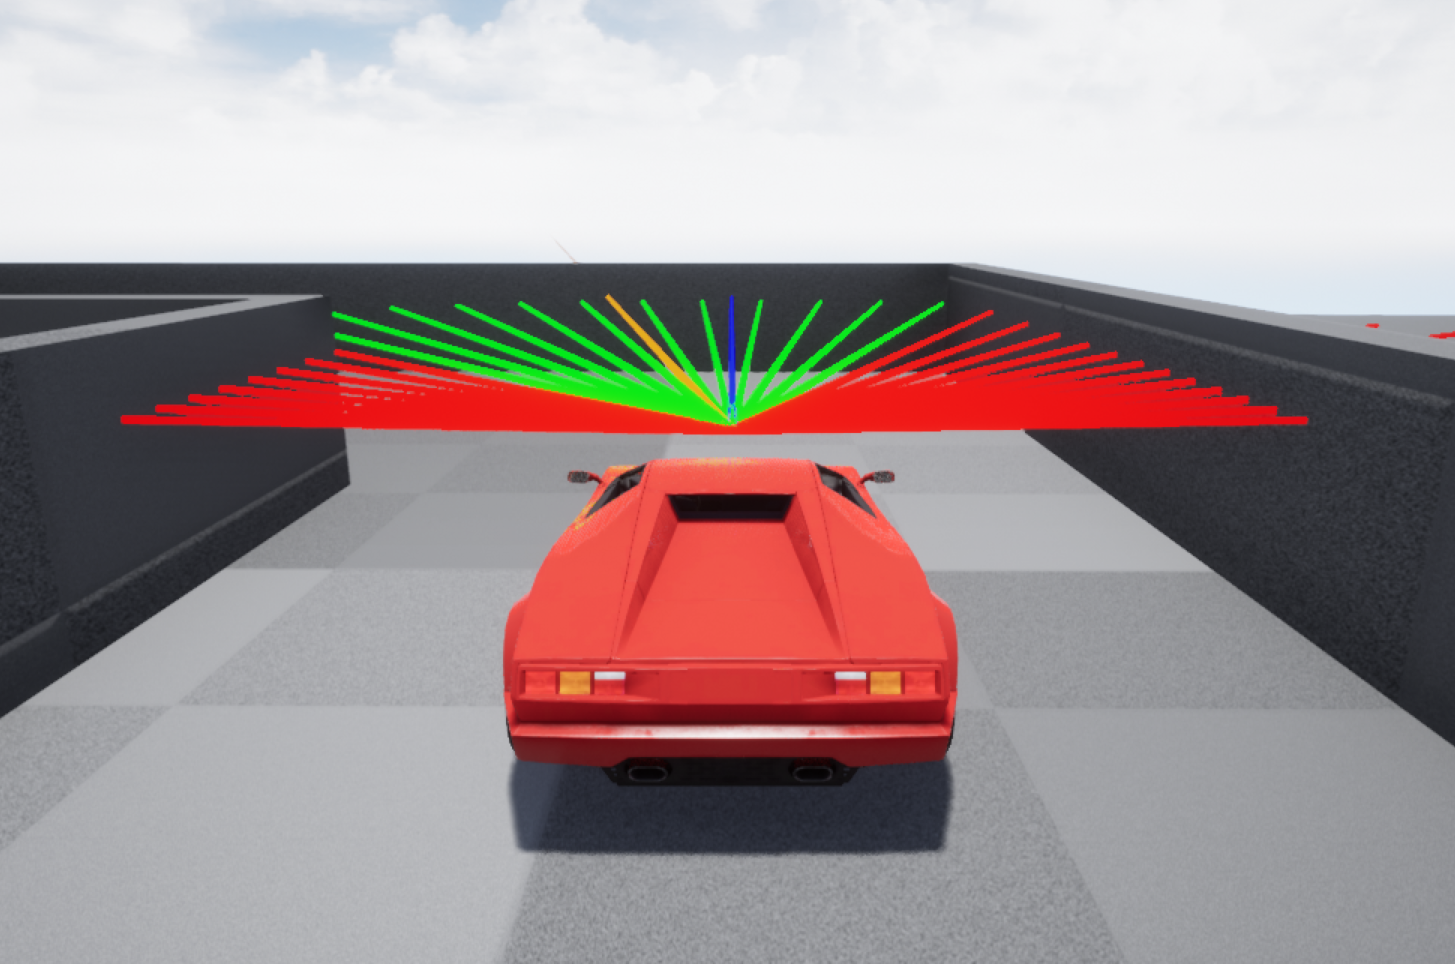
\includegraphics[width=0.7\textwidth]{./Image/State/carSensors.png}
		\vspace{5mm}
		\caption{The image shows how the agent senses the world around it. It is possible to see the $32$ beams equally spaced on a $170^{\circ}$ range. \\
		The beam's color depends wether the ray has hit an obstacle or not: red object is near enough, green no hit. \\
		There are also two other beams (yellow and blue) but they are only for visual puposes, in particular to make humans understand how the agent learns; these will be used in the Reward Fuction \ref{rewardfuc}.}
	\end{figure}
	}\fi
	
	
	\subsection{Policy}
	\sp
	The policy, as mentioned early, is a mapping from state to action, how the agent chooses an action. The goal is to improve the policy over time in order to increase the cumulative reward. \pp
	
	As common in Reinforcement Learning, the agent needs to explore the enviroment to get to know the world around it and after some time then apply this knowledge.  This is known as the \textbf{exploration-exploitation trade-off}: at the begging the agent chooses random actions (exploration), after it has learnt it uses what it knows to choose the correct action (exploitation). \pp
	This exploration-exploitation trade-off is implemented with a value $\epsilon$ commonly initialized to $1$: at each step a random value $c$ (with $c \in [0,1]$) is drawn, if $c\leq\epsilon$ then the agent chooses a random action and $\epsilon$ is decreased otherwise it select the action $a$ with the maximum Q-value given the current state $s$ ($\text{max}_{a}Q_{\theta}(s,a)$).
	\\
	The value of $\epsilon$ is decresed with a value $epsilon\_decay = 7.5 \cdot 10^{-5}$; once $\epsilon$ keep decreasing the probability that $c\leq\epsilon$ will be lower so preferring exploitation over exploration. This is know as \textbf{Epsilon greedy strategy}.\\
	The $epsilon\_decay$ is an hyper-parameter: the lower $epsilon\_decay$ is the more the agent will explore the enviroment increasing the training time. 
	\pp
	The performance of the policy depends on the neural network structure. In this project 3 different architecture are used. %The idea behind them is similar what changes is how the next target Q-value is calculated.; so basically the Bellman equation changes.
	
	\subsubsection{Deep Q-Network}
	\sp
	As mentioned early Deep Q-networks use a neural network to calculate the Q-values given a state and they use \ref{eq:2} to calculate the next Q-value; in particular the target value is calculated with formula \ref{eq:target}, here reported:
	\[
\text{target}_i = r_i + \gamma\text{max}_{a_i^\prime}Q_{\theta}(s_i^{\prime},a_i^{\prime})
\]
and the loss:
\[\mathbb{E}_{(s,a,r,s^\prime)}[(Q_{\theta}(s_i,a_i) - \text{target}_i)^2\] 

	One possible problem with this implementation is that both the current Q-value ($Q_{\theta}(s_i,a_i)$) and the next best Q-value ($\text{max}_{a_i^\prime}Q_{\theta}(s_i^{\prime},a_i^{\prime}$) are calculated using the same network ($Q_{\theta}$). This can bring to overestimations of the values, resulting in overoptimistic value estimates. (add reference)
	
\tikzset{%
  every neuron/.style={
    circle,
    draw,
    minimum size=1cm
  },
  neuron missing/.style={
    draw=none, 
    scale=4,
    text height=0.333cm,
    execute at begin node=\color{black}$\vdots$
  },
}

	
	One possible solution is to use a Double Deep Q-network.
	
	\subsubsection{Double Deep Q-Network} \label{DDQN}
	\sp
	In Double Deep Q-learning 2 networks are used: $Q_{\theta}$ (policy network) and $Q_{\theta^{-}}$ (target network). The 2 networks have the same structure and the weights are initialized with the same values using a RandomNormal kernel initializer. \\
	In this case target and loss are calculated as follow:
	\[
\text{target}_i = r_i + \gamma\text{max}_{a_i^\prime}Q_{\theta^{-}}(s_i^{\prime},a_i^{\prime})
\]
\[\mathbb{E}_{(s,a,r,s^\prime)}[(Q_{\theta}(s_i,a_i) - \text{target}_i)^2\] 
With this solution current Q-value ($Q_{\theta}(s_i,a_i)$) and the next best Q-value ($\text{max}_{a_i^\prime}Q_{\theta^{-}}(s_i^{\prime},a_i^{\prime}$) are calculated using the 2 different networks ($Q_{\theta}$ and $Q_{\theta^{-}}$). This reduces the bias and increases the score.
\\
Over time the loss between $Q_{\theta}$ and $Q_{\theta^{-}}$ is minimized. The weights of network $Q_{\theta}$ are updated every step using the gradient descent formula while the target network's weights ($Q_{\theta^{-}}$) are update every N steps using Polyak averaging: 
\[ \theta^{-} = \tau\theta + (1-\tau)\theta^{-} \]
This is a soft averaging (an hard averaging would be $\theta^{-}=\theta$) weighted by the value $\tau$. $\tau$ represents how much information it has to be kept from the policy network ($\tau=1$ only the information of the policy network, $\tau=0$ only the information of the target network is keep, no update in this case). \cite{DDQN1,DDQN2}
\pp
Both N and $\tau$ are hyper-parameters, in this project they are $N=64$ and $\tau=0.99$

	\subsubsection{Duelling Double Deep Q-Network}
	%http://proceedings.mlr.press/v48/wangf16.pdf
	\sp
	The Q-value Q(s,a) tells us how good it is to take an action a being at state s. This Q-value can be decomposed as the sum of $V(s)$, the value of being at that state, and $A(s,a)$, the advantage of taking that action at the state (from all other possible actions). Mathematically, we can write this as:
	\[ Q(s,a) = V(s) + A(s,a)\]
Dueling Deep Q-network uses two separate estimators for these two components which are then combined together through a special aggregation layer to get an estimate of Q(s,a). By decoupling the estimation, intuitively the Dueling DQN can learn which states are (or are not) valuable without having to learn the effect of each action at each state. This is particularly useful for states where actions do not affect the environment in a meaningful way. \cite{DDQN2} %In these cases, it is unnecessary to evaluate each action for such states and could be skipped to speed up the learning process.
	
The key insight behind this architecture is that for many states, it is unnecessary to es- timate the value of each action choice. For example, in the Enduro game setting \cite{Enduro}, knowing whether to move left or right only matters when a collision is imminent. In some states, it is of paramount importance to know which action to take, but in many other states the choice of action has no repercussion on what happens. For bootstrapping based algorithms, however, the estimation of state values is of great importance for every state \cite{DDDQN1}. 

With this implementation, the Q-value estimate can be obtained by aggregation:
\[ Q(s,a) = V_{\beta}(s) + A_{\alpha}(s,a) - \frac{1}{|A|} \sum_{a^{\prime}}{A_{\alpha}(s,a^{\prime})}\]
where $\beta$ and $\alpha$ are the weights for the networks $V(s)$ and $A(s,a)$ respectively.
	Training of the dueling architectures, as with standard Q-networks, requires only back-propagation. The estimates $V(s)$ and $A(s,a)$ are computed automatically without any extra supervision or algorithmic modifications. In particular this network share the same $N$ and $\tau$ as the Double Deep Q-network \ref{DDQN}
	
	
	
	\subsection{Reward Fuction} \label{rewardfuc}
	\sp
	\subsection{Actions}
	\sp

\end{flushleft}

\newpage
\begin{center}
	\section{Results}
	\sp
\end{center}
\begin{flushleft}
%Specifically, results show interesting zero-shot transferability of a trained agent in the context of (i) inter-city generalization (i.e., the agent is trained on one city and directly applied to another)
\end{flushleft}

\newpage
\begin{center}
	\section{Conclusion}
	\sp
\end{center}
\begin{flushleft}

This internship was a formative experience that allowed me to discover many new topics but also to understand how a company works. Moreover, it allowed me to understand that there is a substantial difference between the university environment and the corporate environment: university, as mentioned by some professors during the courses, has the task of giving a general knowledge of the topics and the real task is to give a way of thinking and analysing a problem to find a solution; indeed, during this period in the company I realized that computer knowledge was not always essential but it was more important to understand what was needed to be done and how to do it.
\ppn

I believe that this internship was very useful because it allowed me to deepen and learn about new topics and gave me an idea to understand if the tasks assigned could be addressed in a future university career or in a possible job.
\newline
This is also an experience that allows to grow both personally and professionally, not to mention that it is a way to
enrich the Curriculum Vitae.

\ppn
I am fully satisfied with the internship as AI researcher and developer and I am satisfied with the atmosphere of serenity and professionalism that I lived in the company thanks to the kind and extremely helpful colleagues.
	\ss
\end{flushleft}

%References
\newpage
\section{References}
\begingroup
\renewcommand{\section}[2]{}
\begin{thebibliography}{999}
\bibitem{AVfirm}
  Todd Litman. 2021.
  \emph{Autonomous Vehicle Implementation Predictions}.\\
  \url{https://www.vtpi.org/avip.pdf}
  
   \bibitem{AVtaxonomy}
  SAE. 2016.
  \emph{Taxonomy and Definitions for Terms Related to Driving Automation Systems for On-Road Motor Vehicles}.\\
  \url{https://www.sae.org/standards/content/j3016_201806/}
   
  \bibitem{AVlevels}
  Monika Stoma, Agnieszka Dudziak, Jacek Caban and Paweł Drozdzie. 2021.
  \emph{The Future of Autonomous Vehicles in the Opinion of Automotive
Market Users}.\\
  \url{https://www.mdpi.com/1996-1073/14/16/4777/pdf}
   
   \bibitem{AVlevels2}
  Piotr CZECH, Katarzyna TUROŃ, Jacek BARCIK. 2018.
  \emph{AUTONOMOUS VEHICLES: BASIC ISSUES}.\\
  \url{https://doi.org/10.20858/sjsutst.2018.100.2}
  
     \bibitem{AVparking}
  Paul Barter. 2013.
  \emph{"Cars are parked 95\% of the time". Let's check!}.\\
  \url{https://www.reinventingparking.org/2013/02/cars-are-parked-95-of-time-lets-check.html}
  
   \bibitem{AVbenefit}
  Jeremy A. Carp. 2018.
  \emph{AUTONOMOUS VEHICLES: PROBLEMS AND PRINCIPLES FOR FUTURE REGULATION}.\\
  \url{https://scholarship.law.upenn.edu/cgi/viewcontent.cgi?article=1048&context=jlpa}
 
   \bibitem{RLandSL}
  ANDREW G. BARTO and THOMAS G. DIETTERICH.
  \emph{Reinforcement Learning and its Relationship to Supervised Learning}.\\
  \url{http://web.engr.orst.edu/~tgd/publications/Barto-Dietterich-03.pdf}
  
  \bibitem{RLapplications}
  Yuxi Li. 2019.
  \emph{REINFORCEMENT LEARNING APPLICATIONS}.\\
  \url{https://arxiv.org/pdf/1908.06973.pdf}
  
  \bibitem{TDl}
  Scholarpedia.org
  \emph{Temporal difference learning}.\\
  \url{http://www.scholarpedia.org/article/Temporal_difference_learning}
 
  \bibitem{Blender}
  \emph{Blender}.\\
  \url{https://www.blender.org/}
   
     \bibitem{UE4}
  \emph{Unreal Engine 4}.\\
  \url{https://www.unrealengine.com/}
   
   
   \bibitem{VVp}
  \emph{Vehicle Variety Pack}.\\
  \url{https://www.unrealengine.com/marketplace/en-US/product/bbcb90a03f844edbb20c8b89ee16ea32}
  
     \bibitem{Lidar}
  \emph{LIDAR}.\\
  \url{https://en.wikipedia.org/wiki/Lidar}
  
  \bibitem{DDQN1}
  Hado van Hasselt and Arthur Guez and David SilverGoogle DeepMind. 2015.
  \emph{Deep Reinforcement Learning with Double Q-learning}.\\
  \url{  https://arxiv.org/pdf/1509.06461.pdf}
   \bibitem{DDQN2}
  Swagat Kumar. 2020.
  \emph{Balancing a CartPole System with Reinforcement Learning}.\\
  \url{https://arxiv.org/pdf/2006.04938v2.pdf}
 
 
  \bibitem{Enduro}
  	Atari 2600. 1983.
  \emph{Enduro (video game)}.\\
  \url{https://en.wikipedia.org/wiki/Enduro_(video_game)}
  \bibitem{DDDQN1}
  	Ziyu Wang, Tom Schaul, Matteo Hessel, Hado van Hasselt, Marc Lanctot, Nando de Freitas. Google DeepMind, London, UK. 2015.
  \emph{Dueling Network Architectures for Deep Reinforcement Learning}.\\
  \url{https://en.wikipedia.org/wiki/Enduro_(video_game)}
   

\end{thebibliography}

\end{document}
